\chapter{Introduction}
\section{Overview}
Obstacle k-Nearest Neighbor (OkNN) is a common type
of spatial analysis query which can be described as follows:
given a set of target points and a collection of polygonal obstacles,
all in two dimensions, find the k closest targets to
an a priori unknown query point q. Such problems appear
in a myriad of practical contexts. For example, in an industrial
warehouse setting a machine operator may be interested
to know the k closest storage locations where a specific inventory
item can be found. OkNN also appears in AI path planning field, for example,
in competitive computer games, agent AIs often rely on nearest-neighbour information
to make strategic decisions such as during navigation,
combat or resource gathering.

\begin{figure}[htp]
  \centering
  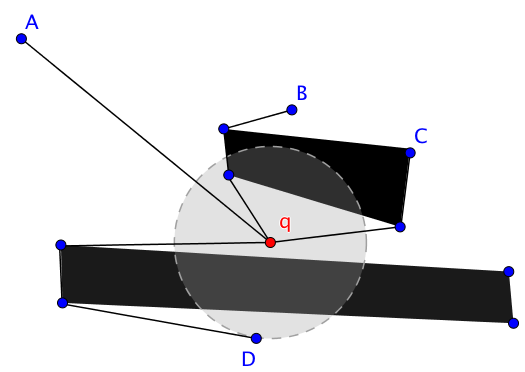
\includegraphics[width=.7\linewidth]{./pic/obs_dis.png}
  \caption{\small
  We aim to find the nearest neighbour of point $q$ from among the set of target points $A,B,C,D$.
  Black lines indicate the Euclidean shortest paths from $q$.
  Notice $D$ is the nearest neighbor of $q$ under the Euclidean metric
  but also the furthest neighbor of $q$ when obstacles are considered.}
\label{obs_dis}
\end{figure}

Tradional kNN queries in the plane (i.e. no obstacles) is a well studied problem that can be
handled by algorithms based on spatial index. A key ingredient to the success of
these algorithms is the Euclidean metric which provides perfect distance information between
any pair of points. When obstacles are introduced however the Euclidean metric becomes an often
misleading lower-bound, and the metric becomes obstacle distance. Figure~\ref{obs_dis} shows such an example.

\section{Major Challenges}
Two popular algorithms for OkNN, which can deal with obstacles, are
\emph{local visibility graphs}~\cite{zhang2004spatial} and \emph{fast
filter}~\cite{xia2004fast}. Though different in details, both of these methods
are similar in that they depend on the incremental and online construction of 
a graph of co-visible points, and use \textit{Dijkstra} to compute shortest path.
Algorithms of this type are simple to understand, 
provide optimality guarantees and the promise of fast performance. 
Such advantages make incremental visibility graphs attractive to researchers 
and, despite more than a decade since their introduction, they continue to 
appear as ingredients in a variety of kNN studies from the literature; e.g. 
~\cite{gao2011efficient,gao2016reverse,gao2009continuous}.
However, incremental visibility graphs also suffer from a number of notable 
disadvantages including:

\begin{enumerate}
  \item online visibility checks;
  \item an incremental construction process that has up to quadratic space and time complexity for the worst case;
  \item duplicated effort, since the graph is discarded each time the query 
  point changes.
\end{enumerate}

In section~\ref{lrknn}, we will introduce these two algorithms with detail,
and discuss why they have such disadvantages.

\section{Major Objectives}
In this research, we develop a new method for computing \emph{OkNN} which avoids same
disadvantages in existing works. Our research extends an existing very fast point-to-point
pathfinding algorithm \emph{Polyanya} to multi-target case.

\section{Thesis Organisation}
The rest of the thesis is organised as follows:
\begin{itemize}
  \item In chapter~\ref{lreview}, we review related works in different area, includes: AI
    searching, spatial index and spatial query processing.
  \item In chapter~\ref{proposedalgo}, we introduce the proposed algorithms and discuss their
    behaviors, formal proof for correctness will be proveded.
  \item In chapter~\ref{empirical}, we provide experiment results to demonstrate the
    performance of propsed algorithms.
  \item In chapter~\ref{conclusionfuture}, we summarize our contributions and discuss future
    works.
\end{itemize}
